\documentclass{article}

\usepackage{graphicx}
\usepackage{amsmath}
\usepackage{lipsum}
\usepackage{multicol,caption}
\usepackage{fullpage}
\usepackage{url}
\usepackage{tabularx}
\usepackage{tabu}

\newenvironment{Figure}
  {\par\medskip\noindent\minipage{\linewidth}}
  {\endminipage\par\medskip}

\begin{document}

\title{$^1S_0$ nucleon-nulceon phase shift with effective field theory -- Report for Project \#2}
\author{}
\date{\today}

\maketitle

\begin{abstract}

\end{abstract}

\begin{multicols}{2}

\section{Introduction}

\section{Pionless Effective Field Theory (EFT)}

\subsection{Leading Order (LO) pionless effective field potential for $^1S_0$}

\subsection{NLO and NNLO correction terms}

\subsection{Inclusion of the \emph{one-pion exchange} (OPE) term}

\section{Results of $^{1}S_{0}$ nucleon-nucleon phase shifts}

\subsection{pionless EFT}

\subsubsection{LO, NLO, NNLO phase shifts}

\begin{Figure}
\centering
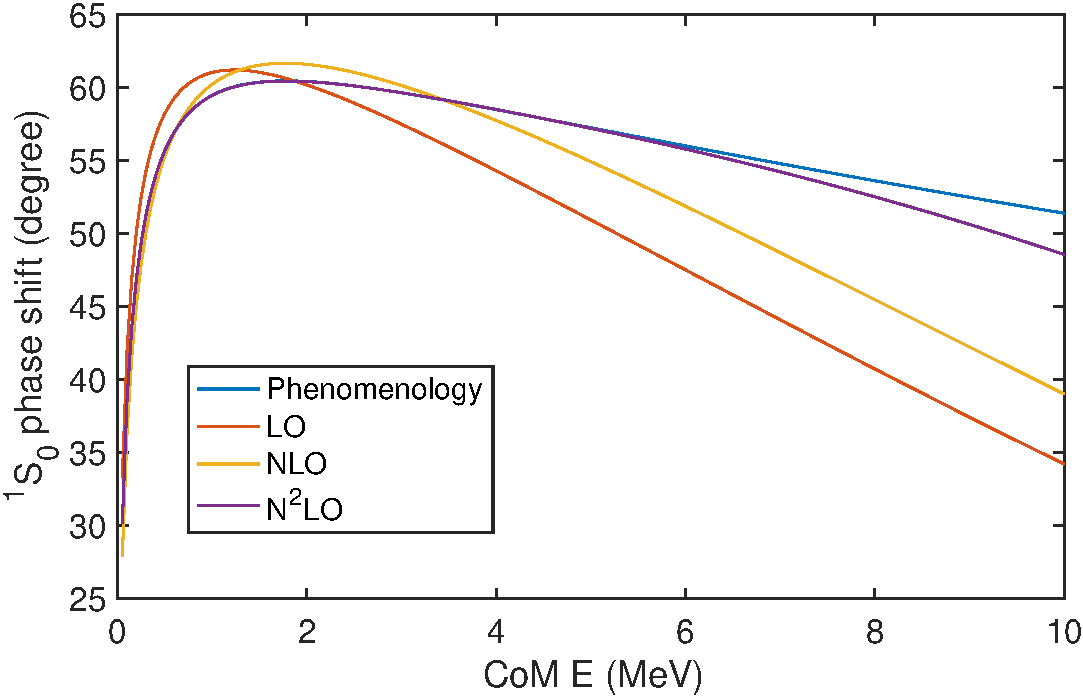
\includegraphics[width=\textwidth]{ps1.pdf}
\captionof{figure}{}
\end{Figure}

\begin{Figure}
\centering
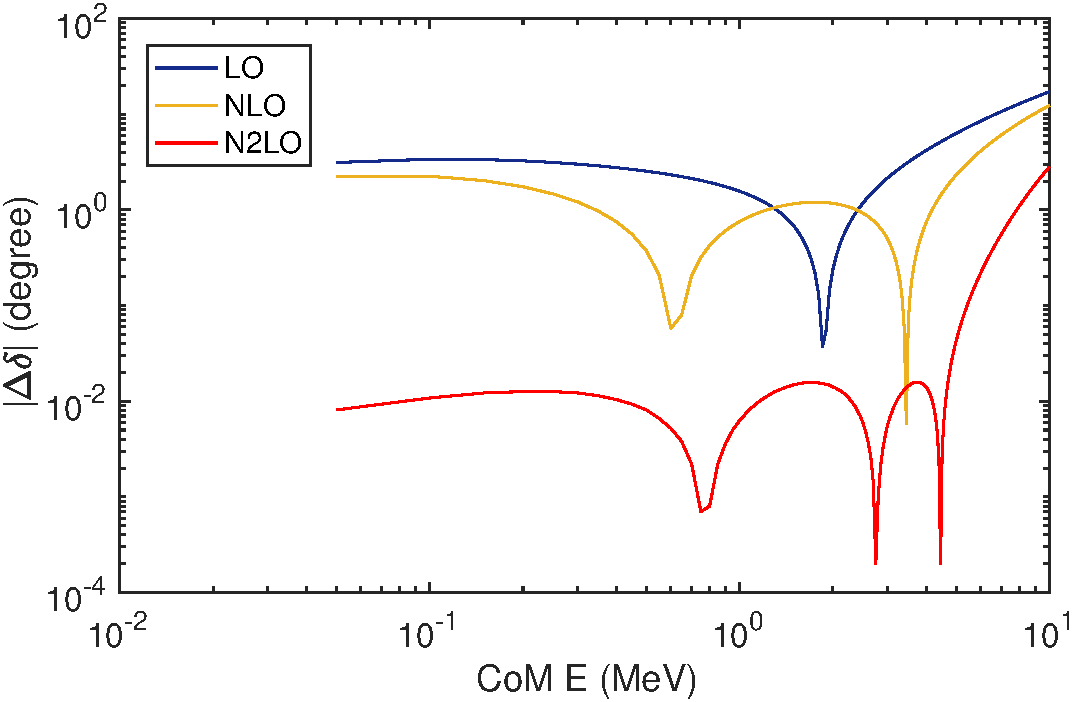
\includegraphics[width=\textwidth]{ps_diff1.pdf}
\captionof{figure}{}
\end{Figure}

\subsubsection{$\Lambda$ cuf-off dependence for NLO}

\begin{Figure}
\centering
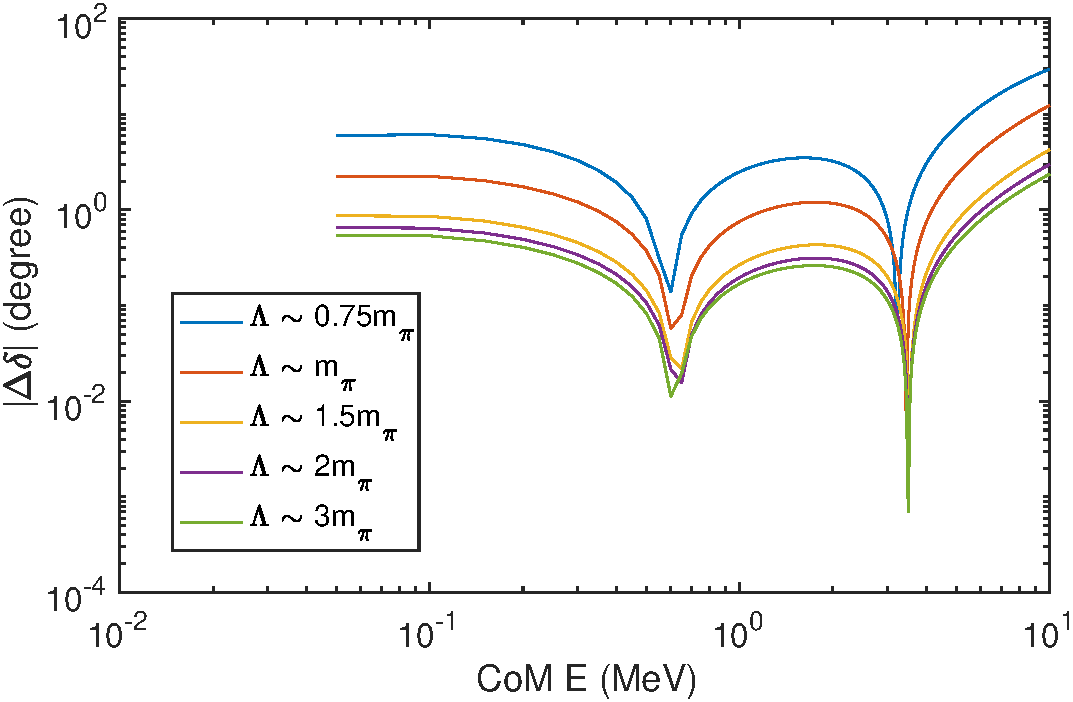
\includegraphics[width=\textwidth]{partc.pdf}
\captionof{figure}{}
\end{Figure}

\subsection{pionless EFT with a phenomenological OPE potential}

\subsubsection{LO, NLO, NNLO phase shifts}

\begin{Figure}
\centering
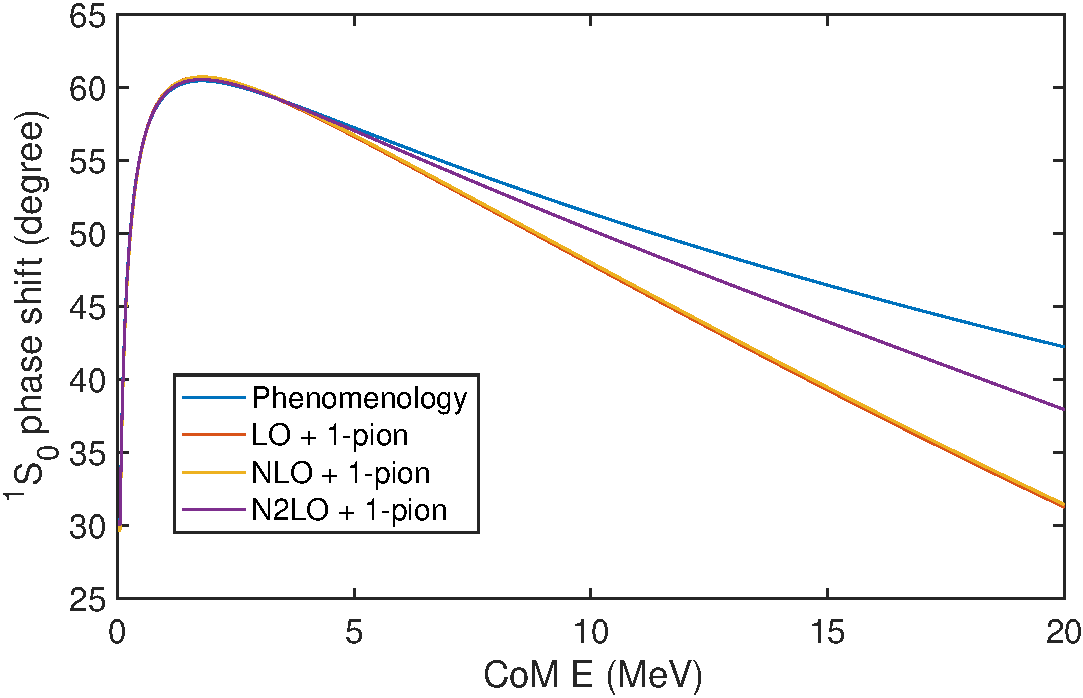
\includegraphics[width=\textwidth]{ps2.pdf}
\captionof{figure}{}
\end{Figure}

\begin{Figure}
\centering
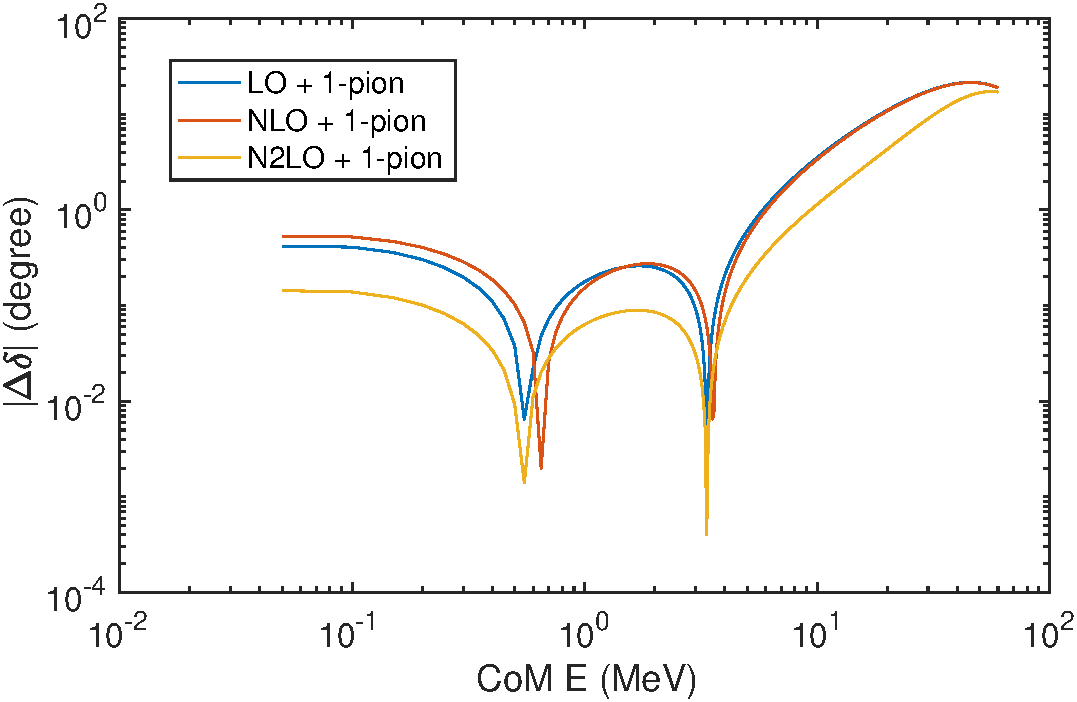
\includegraphics[width=\textwidth]{ps_diff2.pdf}
\captionof{figure}{}
\end{Figure}

\section{Conclusion}

\end{multicols}

\hrulefill

\begin{enumerate} % References

\item S. Bogner and M. Hjorth-Jensen, \textit{Project 1 Assignment Notes}, \url{https://manybodyphysics.github.io/NuclearForces/doc/web/course.html}

\item S. Bogner and M. Hjorth-Jensen, \textit{Project 2 Assignment Notes}, \url{https://manybodyphysics.github.io/NuclearForces/doc/Projects/2017/Project2/pdf/Project2.pdf}

\end{enumerate}

\end{document}
